\documentclass[1p]{elsarticle_modified}
%\bibliographystyle{elsarticle-num}

%\usepackage[colorlinks]{hyperref}
%\usepackage{abbrmath_seonhwa} %\Abb, \Ascr, \Acal ,\Abf, \Afrak
\usepackage{amsfonts}
\usepackage{amssymb}
\usepackage{amsmath}
\usepackage{amsthm}
\usepackage{scalefnt}
\usepackage{amsbsy}
\usepackage{kotex}
\usepackage{caption}
\usepackage{subfig}
\usepackage{color}
\usepackage{graphicx}
\usepackage{xcolor} %% white, black, red, green, blue, cyan, magenta, yellow
\usepackage{float}
\usepackage{setspace}
\usepackage{hyperref}

\usepackage{tikz}
\usetikzlibrary{arrows}

\usepackage{multirow}
\usepackage{array} % fixed length table
\usepackage{hhline}

%%%%%%%%%%%%%%%%%%%%%
\makeatletter
\renewcommand*\env@matrix[1][\arraystretch]{%
	\edef\arraystretch{#1}%
	\hskip -\arraycolsep
	\let\@ifnextchar\new@ifnextchar
	\array{*\c@MaxMatrixCols c}}
\makeatother %https://tex.stackexchange.com/questions/14071/how-can-i-increase-the-line-spacing-in-a-matrix
%%%%%%%%%%%%%%%

\usepackage[normalem]{ulem}

\newcommand{\msout}[1]{\ifmmode\text{\sout{\ensuremath{#1}}}\else\sout{#1}\fi}
%SOURCE: \msout is \stkout macro in https://tex.stackexchange.com/questions/20609/strikeout-in-math-mode

\newcommand{\cancel}[1]{
	\ifmmode
	{\color{red}\msout{#1}}
	\else
	{\color{red}\sout{#1}}
	\fi
}

\newcommand{\add}[1]{
	{\color{blue}\uwave{#1}}
}

\newcommand{\replace}[2]{
	\ifmmode
	{\color{red}\msout{#1}}{\color{blue}\uwave{#2}}
	\else
	{\color{red}\sout{#1}}{\color{blue}\uwave{#2}}
	\fi
}

\newcommand{\Sol}{\mathcal{S}} %segment
\newcommand{\D}{D} %diagram
\newcommand{\A}{\mathcal{A}} %arc


%%%%%%%%%%%%%%%%%%%%%%%%%%%%%5 test

\def\sl{\operatorname{\textup{SL}}(2,\Cbb)}
\def\psl{\operatorname{\textup{PSL}}(2,\Cbb)}
\def\quan{\mkern 1mu \triangleright \mkern 1mu}

\theoremstyle{definition}
\newtheorem{thm}{Theorem}[section]
\newtheorem{prop}[thm]{Proposition}
\newtheorem{lem}[thm]{Lemma}
\newtheorem{ques}[thm]{Question}
\newtheorem{cor}[thm]{Corollary}
\newtheorem{defn}[thm]{Definition}
\newtheorem{exam}[thm]{Example}
\newtheorem{rmk}[thm]{Remark}
\newtheorem{alg}[thm]{Algorithm}

\newcommand{\I}{\sqrt{-1}}
\begin{document}

%\begin{frontmatter}
%
%\title{Boundary parabolic representations of knots up to 8 crossings}
%
%%% Group authors per affiliation:
%\author{Yunhi Cho} 
%\address{Department of Mathematics, University of Seoul, Seoul, Korea}
%\ead{yhcho@uos.ac.kr}
%
%
%\author{Seonhwa Kim} %\fnref{s_kim}}
%\address{Center for Geometry and Physics, Institute for Basic Science, Pohang, 37673, Korea}
%\ead{ryeona17@ibs.re.kr}
%
%\author{Hyuk Kim}
%\address{Department of Mathematical Sciences, Seoul National University, Seoul 08826, Korea}
%\ead{hyukkim@snu.ac.kr}
%
%\author{Seokbeom Yoon}
%\address{Department of Mathematical Sciences, Seoul National University, Seoul, 08826,  Korea}
%\ead{sbyoon15@snu.ac.kr}
%
%\begin{abstract}
%We find all boundary parabolic representation of knots up to 8 crossings.
%
%\end{abstract}
%\begin{keyword}
%    \MSC[2010] 57M25 
%\end{keyword}
%
%\end{frontmatter}

%\linenumbers
%\tableofcontents
%
\newcommand\colored[1]{\textcolor{white}{\rule[-0.35ex]{0.8em}{1.4ex}}\kern-0.8em\color{red} #1}%
%\newcommand\colored[1]{\textcolor{white}{ #1}\kern-2.17ex	\textcolor{white}{ #1}\kern-1.81ex	\textcolor{white}{ #1}\kern-2.15ex\color{red}#1	}

{\Large $\underline{12n_{0695}~(K12n_{0695})}$}

\setlength{\tabcolsep}{10pt}
\renewcommand{\arraystretch}{1.6}
\vspace{1cm}\begin{tabular}{m{100pt}>{\centering\arraybackslash}m{274pt}}
\multirow{5}{120pt}{
	\centering
	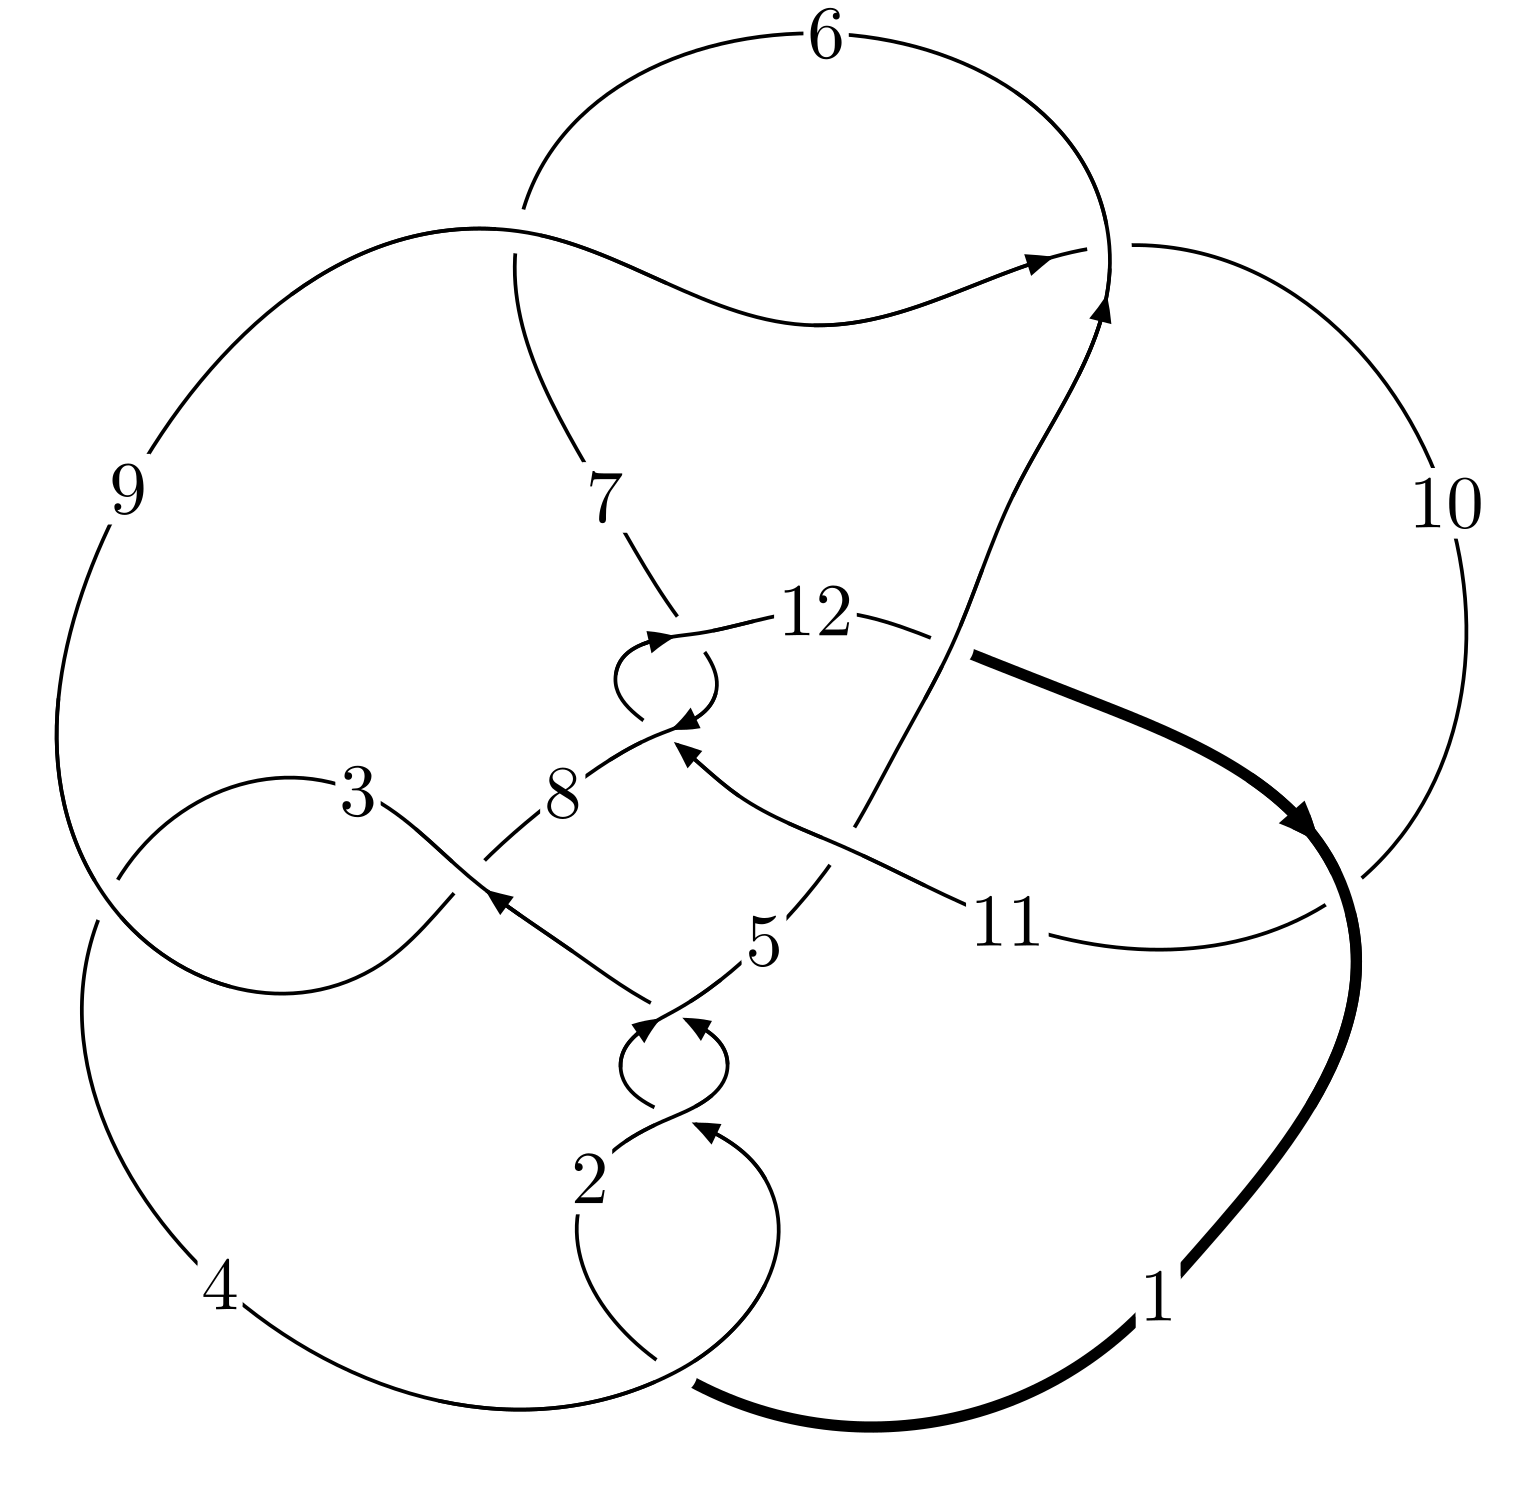
\includegraphics[width=112pt]{../../../GIT/diagram.site/Diagrams/png/2784_12n_0695.png}\\
\ \ \ A knot diagram\footnotemark}&
\allowdisplaybreaks
\textbf{Linearized knot diagam} \\
\cline{2-2}
 &
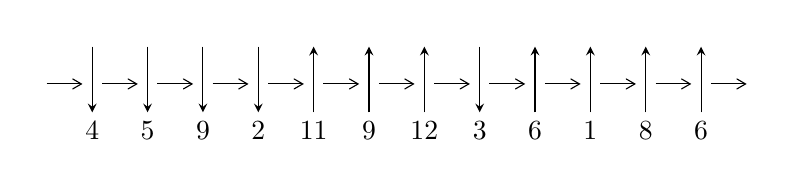
\begin{tikzpicture}[x=20pt, y=17pt]
	% nodes
	\node (C0) at (0, 0) {};
	\node (C1) at (1, 0) {};
	\node (C1U) at (1, +1) {};
	\node (C1D) at (1, -1) {4};

	\node (C2) at (2, 0) {};
	\node (C2U) at (2, +1) {};
	\node (C2D) at (2, -1) {5};

	\node (C3) at (3, 0) {};
	\node (C3U) at (3, +1) {};
	\node (C3D) at (3, -1) {9};

	\node (C4) at (4, 0) {};
	\node (C4U) at (4, +1) {};
	\node (C4D) at (4, -1) {2};

	\node (C5) at (5, 0) {};
	\node (C5U) at (5, +1) {};
	\node (C5D) at (5, -1) {11};

	\node (C6) at (6, 0) {};
	\node (C6U) at (6, +1) {};
	\node (C6D) at (6, -1) {9};

	\node (C7) at (7, 0) {};
	\node (C7U) at (7, +1) {};
	\node (C7D) at (7, -1) {12};

	\node (C8) at (8, 0) {};
	\node (C8U) at (8, +1) {};
	\node (C8D) at (8, -1) {3};

	\node (C9) at (9, 0) {};
	\node (C9U) at (9, +1) {};
	\node (C9D) at (9, -1) {6};

	\node (C10) at (10, 0) {};
	\node (C10U) at (10, +1) {};
	\node (C10D) at (10, -1) {1};

	\node (C11) at (11, 0) {};
	\node (C11U) at (11, +1) {};
	\node (C11D) at (11, -1) {8};

	\node (C12) at (12, 0) {};
	\node (C12U) at (12, +1) {};
	\node (C12D) at (12, -1) {6};
	\node (C13) at (13, 0) {};

	% arrows
	\draw[->,>={angle 60}]
	(C0) edge (C1) (C1) edge (C2) (C2) edge (C3) (C3) edge (C4) (C4) edge (C5) (C5) edge (C6) (C6) edge (C7) (C7) edge (C8) (C8) edge (C9) (C9) edge (C10) (C10) edge (C11) (C11) edge (C12) (C12) edge (C13) ;	\draw[->,>=stealth]
	(C1U) edge (C1D) (C2U) edge (C2D) (C3U) edge (C3D) (C4U) edge (C4D) (C5D) edge (C5U) (C6D) edge (C6U) (C7D) edge (C7U) (C8U) edge (C8D) (C9D) edge (C9U) (C10D) edge (C10U) (C11D) edge (C11U) (C12D) edge (C12U) ;
	\end{tikzpicture} \\
\hhline{~~} \\& 
\textbf{Solving Sequence} \\ \cline{2-2} 
 &
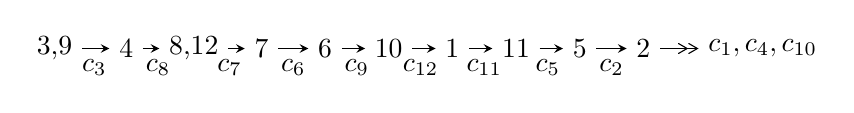
\begin{tikzpicture}[x=23pt, y=7pt]
	% node
	\node (A0) at (-1/8, 0) {3,9};
	\node (A1) at (1, 0) {4};
	\node (A2) at (33/16, 0) {8,12};
	\node (A3) at (25/8, 0) {7};
	\node (A4) at (33/8, 0) {6};
	\node (A5) at (41/8, 0) {10};
	\node (A6) at (49/8, 0) {1};
	\node (A7) at (57/8, 0) {11};
	\node (A8) at (65/8, 0) {5};
	\node (A9) at (73/8, 0) {2};
	\node (C1) at (1/2, -1) {$c_{3}$};
	\node (C2) at (3/2, -1) {$c_{8}$};
	\node (C3) at (21/8, -1) {$c_{7}$};
	\node (C4) at (29/8, -1) {$c_{6}$};
	\node (C5) at (37/8, -1) {$c_{9}$};
	\node (C6) at (45/8, -1) {$c_{12}$};
	\node (C7) at (53/8, -1) {$c_{11}$};
	\node (C8) at (61/8, -1) {$c_{5}$};
	\node (C9) at (69/8, -1) {$c_{2}$};
	\node (A10) at (11, 0) {$c_{1},c_{4},c_{10}$};

	% edge
	\draw[->,>=stealth]	
	(A0) edge (A1) (A1) edge (A2) (A2) edge (A3) (A3) edge (A4) (A4) edge (A5) (A5) edge (A6) (A6) edge (A7) (A7) edge (A8) (A8) edge (A9) ;
	\draw[->>,>={angle 60}]	
	(A9) edge (A10);
\end{tikzpicture} \\ 

\end{tabular} \\

\footnotetext{
The image of knot diagram is generated by the software ``\textbf{Draw programme}" developed by Andrew Bartholomew(\url{http://www.layer8.co.uk/maths/draw/index.htm\#Running-draw}), where we modified some parts for our purpose(\url{https://github.com/CATsTAILs/LinksPainter}).
}\phantom \\ \newline 
\centering \textbf{Ideals for irreducible components\footnotemark of $X_{\text{par}}$} 
 
\begin{align*}
I^u_{1}&=\langle 
-1.13964\times10^{33} u^{26}-5.99682\times10^{33} u^{25}+\cdots+3.81255\times10^{34} b-2.47902\times10^{35},\\
\phantom{I^u_{1}}&\phantom{= \langle  }-2.08631\times10^{34} u^{26}-1.00367\times10^{35} u^{25}+\cdots+7.62510\times10^{34} a-4.15461\times10^{36},\\
\phantom{I^u_{1}}&\phantom{= \langle  }u^{27}+5 u^{26}+\cdots+400 u+64\rangle \\
I^u_{2}&=\langle 
176363 u^{14}+128033 u^{13}+\cdots+74749 b-928241,\;61025 u^{14}+17351 u^{13}+\cdots+74749 a-408316,\\
\phantom{I^u_{2}}&\phantom{= \langle  }u^{15}-3 u^{13}+4 u^{11}-2 u^{10}+u^9+5 u^8-5 u^7-5 u^6- u^5+9 u^4+9 u^3-4 u^2-3 u+1\rangle \\
I^u_{3}&=\langle 
4 u^7-2 u^6-6 u^5+u^2 b a+6 u^4+8 u^3+b^2-2 b a- a u-5 u^2-4 u+7,\\
\phantom{I^u_{3}}&\phantom{= \langle  }- u^7 a+u^6 a-2 u^7+u^5 a+u^6-2 u^4 a+3 u^5- u^3 a-3 u^4+2 u^2 a-4 u^3+a^2+3 u^2-2 a+2 u-4,\\
\phantom{I^u_{3}}&\phantom{= \langle  }u^8- u^7- u^6+2 u^5+u^4-2 u^3+2 u-1\rangle \\
\\
I^v_{1}&=\langle 
a,\;4 b- v+4,\;v^2-6 v+4\rangle \\
\end{align*}
\raggedright * 4 irreducible components of $\dim_{\mathbb{C}}=0$, with total 76 representations.\\
\footnotetext{All coefficients of polynomials are rational numbers. But the coefficients are sometimes approximated in decimal forms when there is not enough margin.}
\newpage
\renewcommand{\arraystretch}{1}
\centering \section*{I. $I^u_{1}= \langle -1.14\times10^{33} u^{26}-6.00\times10^{33} u^{25}+\cdots+3.81\times10^{34} b-2.48\times10^{35},\;-2.09\times10^{34} u^{26}-1.00\times10^{35} u^{25}+\cdots+7.63\times10^{34} a-4.15\times10^{36},\;u^{27}+5 u^{26}+\cdots+400 u+64 \rangle$}
\flushleft \textbf{(i) Arc colorings}\\
\begin{tabular}{m{7pt} m{180pt} m{7pt} m{180pt} }
\flushright $a_{3}=$&$\begin{pmatrix}1\\0\end{pmatrix}$ \\
\flushright $a_{9}=$&$\begin{pmatrix}0\\u\end{pmatrix}$ \\
\flushright $a_{4}=$&$\begin{pmatrix}1\\u^2\end{pmatrix}$ \\
\flushright $a_{8}=$&$\begin{pmatrix}u\\u\end{pmatrix}$ \\
\flushright $a_{12}=$&$\begin{pmatrix}0.273610 u^{26}+1.31627 u^{25}+\cdots+187.951 u+54.4860\\0.0298919 u^{26}+0.157291 u^{25}+\cdots+24.8662 u+6.50226\end{pmatrix}$ \\
\flushright $a_{7}=$&$\begin{pmatrix}0.603225 u^{26}+2.76296 u^{25}+\cdots+357.964 u+98.6342\\-0.0171631 u^{26}-0.0712776 u^{25}+\cdots-6.60142 u-2.12730\end{pmatrix}$ \\
\flushright $a_{6}=$&$\begin{pmatrix}0.603225 u^{26}+2.76296 u^{25}+\cdots+357.964 u+98.6342\\0.106750 u^{26}+0.472111 u^{25}+\cdots+56.0584 u+14.0753\end{pmatrix}$ \\
\flushright $a_{10}=$&$\begin{pmatrix}-1.39047 u^{26}-6.44135 u^{25}+\cdots-854.422 u-239.806\\-0.0213532 u^{26}-0.118447 u^{25}+\cdots-20.2449 u-6.81187\end{pmatrix}$ \\
\flushright $a_{1}=$&$\begin{pmatrix}-1.11686 u^{26}-5.12508 u^{25}+\cdots-666.471 u-185.320\\0.00853870 u^{26}+0.0388446 u^{25}+\cdots+3.62131 u-0.309612\end{pmatrix}$ \\
\flushright $a_{11}=$&$\begin{pmatrix}0.266493 u^{26}+1.31042 u^{25}+\cdots+196.198 u+58.3012\\0.0227747 u^{26}+0.151445 u^{25}+\cdots+33.1133 u+10.3175\end{pmatrix}$ \\
\flushright $a_{5}=$&$\begin{pmatrix}1.34575 u^{26}+6.12897 u^{25}+\cdots+782.304 u+214.401\\0.228884 u^{26}+1.00389 u^{25}+\cdots+115.833 u+29.0810\end{pmatrix}$ \\
\flushright $a_{2}=$&$\begin{pmatrix}-1.34575 u^{26}-6.12897 u^{25}+\cdots-782.304 u-214.401\\-0.0973818 u^{26}-0.399745 u^{25}+\cdots-37.9426 u-9.30362\end{pmatrix}$\\&\end{tabular}
\flushleft \textbf{(ii) Obstruction class $= -1$}\\~\\
\flushleft \textbf{(iii) Cusp Shapes $= -1.27815 u^{26}-5.86437 u^{25}+\cdots-764.039 u-222.235$}\\~\\
\newpage\renewcommand{\arraystretch}{1}
\flushleft \textbf{(iv) u-Polynomials at the component}\newline \\
\begin{tabular}{m{50pt}|m{274pt}}
Crossings & \hspace{64pt}u-Polynomials at each crossing \\
\hline $$\begin{aligned}c_{1},c_{2},c_{4}\end{aligned}$$&$\begin{aligned}
&u^{27}-3 u^{26}+\cdots-36 u+16
\end{aligned}$\\
\hline $$\begin{aligned}c_{3},c_{8}\end{aligned}$$&$\begin{aligned}
&u^{27}+5 u^{26}+\cdots+400 u+64
\end{aligned}$\\
\hline $$\begin{aligned}c_{5},c_{7},c_{11}\end{aligned}$$&$\begin{aligned}
&u^{27}+u^{26}+\cdots-5 u-1
\end{aligned}$\\
\hline $$\begin{aligned}c_{6},c_{9},c_{12}\end{aligned}$$&$\begin{aligned}
&u^{27}-25 u^{25}+\cdots+6 u+1
\end{aligned}$\\
\hline $$\begin{aligned}c_{10}\end{aligned}$$&$\begin{aligned}
&u^{27}+19 u^{26}+\cdots-768 u+256
\end{aligned}$\\
\hline
\end{tabular}\\~\\
\newpage\renewcommand{\arraystretch}{1}
\flushleft \textbf{(v) Riley Polynomials at the component}\newline \\
\begin{tabular}{m{50pt}|m{274pt}}
Crossings & \hspace{64pt}Riley Polynomials at each crossing \\
\hline $$\begin{aligned}c_{1},c_{2},c_{4}\end{aligned}$$&$\begin{aligned}
&y^{27}-23 y^{26}+\cdots-2192 y-256
\end{aligned}$\\
\hline $$\begin{aligned}c_{3},c_{8}\end{aligned}$$&$\begin{aligned}
&y^{27}-9 y^{26}+\cdots+49920 y-4096
\end{aligned}$\\
\hline $$\begin{aligned}c_{5},c_{7},c_{11}\end{aligned}$$&$\begin{aligned}
&y^{27}+5 y^{26}+\cdots+15 y-1
\end{aligned}$\\
\hline $$\begin{aligned}c_{6},c_{9},c_{12}\end{aligned}$$&$\begin{aligned}
&y^{27}-50 y^{26}+\cdots+68 y-1
\end{aligned}$\\
\hline $$\begin{aligned}c_{10}\end{aligned}$$&$\begin{aligned}
&y^{27}-19 y^{26}+\cdots+5636096 y-65536
\end{aligned}$\\
\hline
\end{tabular}\\~\\
\newpage\flushleft \textbf{(vi) Complex Volumes and Cusp Shapes}
$$\begin{array}{c|c|c}  
\text{Solutions to }I^u_{1}& \I (\text{vol} + \sqrt{-1}CS) & \text{Cusp shape}\\
 \hline 
\begin{aligned}
u &= -1.03853\phantom{ +0.000000I} \\
a &= -1.40893\phantom{ +0.000000I} \\
b &= -0.426622\phantom{ +0.000000I}\end{aligned}
 & -2.58509\phantom{ +0.000000I} & -5.21480\phantom{ +0.000000I} \\ \hline\begin{aligned}
u &= -1.162780 + 0.105322 I \\
a &= \phantom{-}0.256922 + 0.751420 I \\
b &= -0.008028 + 1.317420 I\end{aligned}
 & -2.12887 + 0.87840 I & -1.69411 + 0.10409 I \\ \hline\begin{aligned}
u &= -1.162780 - 0.105322 I \\
a &= \phantom{-}0.256922 - 0.751420 I \\
b &= -0.008028 - 1.317420 I\end{aligned}
 & -2.12887 - 0.87840 I & -1.69411 - 0.10409 I \\ \hline\begin{aligned}
u &= -0.152365 + 1.192150 I \\
a &= -0.893744 + 0.183757 I \\
b &= -0.260772 + 0.484211 I\end{aligned}
 & -3.95830 - 1.70076 I & -0.66920 + 3.77891 I \\ \hline\begin{aligned}
u &= -0.152365 - 1.192150 I \\
a &= -0.893744 - 0.183757 I \\
b &= -0.260772 - 0.484211 I\end{aligned}
 & -3.95830 + 1.70076 I & -0.66920 - 3.77891 I \\ \hline\begin{aligned}
u &= \phantom{-}1.153410 + 0.362069 I \\
a &= -0.124158 - 0.993672 I \\
b &= \phantom{-}0.18813 - 1.67407 I\end{aligned}
 & -1.52168 - 4.11639 I & \phantom{-}1.28531 + 7.66399 I \\ \hline\begin{aligned}
u &= \phantom{-}1.153410 - 0.362069 I \\
a &= -0.124158 + 0.993672 I \\
b &= \phantom{-}0.18813 + 1.67407 I\end{aligned}
 & -1.52168 + 4.11639 I & \phantom{-}1.28531 - 7.66399 I \\ \hline\begin{aligned}
u &= \phantom{-}0.550134 + 1.176880 I \\
a &= -0.727410 + 0.882315 I \\
b &= \phantom{-}0.082313 + 0.573084 I\end{aligned}
 & \phantom{-}6.85248 + 3.47221 I & \phantom{-}4.05373 - 4.83355 I \\ \hline\begin{aligned}
u &= \phantom{-}0.550134 - 1.176880 I \\
a &= -0.727410 - 0.882315 I \\
b &= \phantom{-}0.082313 - 0.573084 I\end{aligned}
 & \phantom{-}6.85248 - 3.47221 I & \phantom{-}4.05373 + 4.83355 I \\ \hline\begin{aligned}
u &= -0.450239 + 1.331950 I \\
a &= \phantom{-}0.460049 + 0.710367 I \\
b &= \phantom{-}0.027730 + 0.522672 I\end{aligned}
 & \phantom{-}5.01150 + 2.13942 I & -3.15739 + 7.15620 I\\
 \hline 
 \end{array}$$\newpage$$\begin{array}{c|c|c}  
\text{Solutions to }I^u_{1}& \I (\text{vol} + \sqrt{-1}CS) & \text{Cusp shape}\\
 \hline 
\begin{aligned}
u &= -0.450239 - 1.331950 I \\
a &= \phantom{-}0.460049 - 0.710367 I \\
b &= \phantom{-}0.027730 - 0.522672 I\end{aligned}
 & \phantom{-}5.01150 - 2.13942 I & -3.15739 - 7.15620 I \\ \hline\begin{aligned}
u &= \phantom{-}0.290484 + 0.513132 I \\
a &= \phantom{-}1.005030 - 0.448330 I \\
b &= \phantom{-}0.178104 + 0.233390 I\end{aligned}
 & \phantom{-}1.086740 + 0.522072 I & \phantom{-}7.59034 - 2.64068 I \\ \hline\begin{aligned}
u &= \phantom{-}0.290484 - 0.513132 I \\
a &= \phantom{-}1.005030 + 0.448330 I \\
b &= \phantom{-}0.178104 - 0.233390 I\end{aligned}
 & \phantom{-}1.086740 - 0.522072 I & \phantom{-}7.59034 + 2.64068 I \\ \hline\begin{aligned}
u &= -1.26259 + 0.65120 I \\
a &= \phantom{-}0.779025 + 0.806632 I \\
b &= \phantom{-}0.89947 + 1.69470 I\end{aligned}
 & \phantom{-}1.93276 + 4.57399 I & -0.80312 - 3.71996 I \\ \hline\begin{aligned}
u &= -1.26259 - 0.65120 I \\
a &= \phantom{-}0.779025 - 0.806632 I \\
b &= \phantom{-}0.89947 - 1.69470 I\end{aligned}
 & \phantom{-}1.93276 - 4.57399 I & -0.80312 + 3.71996 I \\ \hline\begin{aligned}
u &= \phantom{-}1.21341 + 0.77536 I \\
a &= -0.786921 + 0.889637 I \\
b &= -0.87894 + 1.94262 I\end{aligned}
 & \phantom{-}4.69053 - 10.38600 I & \phantom{-}1.88291 + 6.53281 I \\ \hline\begin{aligned}
u &= \phantom{-}1.21341 - 0.77536 I \\
a &= -0.786921 - 0.889637 I \\
b &= -0.87894 - 1.94262 I\end{aligned}
 & \phantom{-}4.69053 + 10.38600 I & \phantom{-}1.88291 - 6.53281 I \\ \hline\begin{aligned}
u &= -0.72141 + 1.25819 I \\
a &= \phantom{-}0.852837 + 0.774968 I \\
b &= -0.116207 + 0.690641 I\end{aligned}
 & \phantom{-}1.18821 - 7.91289 I & -0.57657 + 4.83516 I \\ \hline\begin{aligned}
u &= -0.72141 - 1.25819 I \\
a &= \phantom{-}0.852837 - 0.774968 I \\
b &= -0.116207 - 0.690641 I\end{aligned}
 & \phantom{-}1.18821 + 7.91289 I & -0.57657 - 4.83516 I \\ \hline\begin{aligned}
u &= -1.36519 + 0.61368 I \\
a &= \phantom{-}0.190407 - 1.118590 I \\
b &= -0.07359 - 1.82092 I\end{aligned}
 & -7.80864 + 8.10776 I & -0.12578 - 8.54506 I\\
 \hline 
 \end{array}$$\newpage$$\begin{array}{c|c|c}  
\text{Solutions to }I^u_{1}& \I (\text{vol} + \sqrt{-1}CS) & \text{Cusp shape}\\
 \hline 
\begin{aligned}
u &= -1.36519 - 0.61368 I \\
a &= \phantom{-}0.190407 + 1.118590 I \\
b &= -0.07359 + 1.82092 I\end{aligned}
 & -7.80864 - 8.10776 I & -0.12578 + 8.54506 I \\ \hline\begin{aligned}
u &= -1.22422 + 0.88045 I \\
a &= \phantom{-}0.754688 + 0.924811 I \\
b &= \phantom{-}0.75841 + 2.06080 I\end{aligned}
 & -0.5454 + 15.5229 I & -1.18119 - 7.76656 I \\ \hline\begin{aligned}
u &= -1.22422 - 0.88045 I \\
a &= \phantom{-}0.754688 - 0.924811 I \\
b &= \phantom{-}0.75841 - 2.06080 I\end{aligned}
 & -0.5454 - 15.5229 I & -1.18119 + 7.76656 I \\ \hline\begin{aligned}
u &= -0.435512\phantom{ +0.000000I} \\
a &= -0.249742\phantom{ +0.000000I} \\
b &= -0.798841\phantom{ +0.000000I}\end{aligned}
 & -1.27409\phantom{ +0.000000I} & -10.1920\phantom{ +0.000000I} \\ \hline\begin{aligned}
u &= \phantom{-}1.55472 + 0.34572 I \\
a &= -0.514140 + 0.857873 I \\
b &= -0.33875 + 1.54021 I\end{aligned}
 & -9.70709 - 4.18623 I & -3.33842 + 3.07970 I \\ \hline\begin{aligned}
u &= \phantom{-}1.55472 - 0.34572 I \\
a &= -0.514140 - 0.857873 I \\
b &= -0.33875 - 1.54021 I\end{aligned}
 & -9.70709 + 4.18623 I & -3.33842 - 3.07970 I \\ \hline\begin{aligned}
u &= -0.372671\phantom{ +0.000000I} \\
a &= \phantom{-}4.40350\phantom{ +0.000000I} \\
b &= -0.190276\phantom{ +0.000000I}\end{aligned}
 & \phantom{-}7.09486\phantom{ +0.000000I} & -26.8760\phantom{ +0.000000I}\\
 \hline 
 \end{array}$$\newpage\newpage\renewcommand{\arraystretch}{1}
\centering \section*{II. $I^u_{2}= \langle 1.76\times10^{5} u^{14}+1.28\times10^{5} u^{13}+\cdots+7.47\times10^{4} b-9.28\times10^{5},\;61025 u^{14}+17351 u^{13}+\cdots+74749 a-408316,\;u^{15}-3 u^{13}+\cdots-3 u+1 \rangle$}
\flushleft \textbf{(i) Arc colorings}\\
\begin{tabular}{m{7pt} m{180pt} m{7pt} m{180pt} }
\flushright $a_{3}=$&$\begin{pmatrix}1\\0\end{pmatrix}$ \\
\flushright $a_{9}=$&$\begin{pmatrix}0\\u\end{pmatrix}$ \\
\flushright $a_{4}=$&$\begin{pmatrix}1\\u^2\end{pmatrix}$ \\
\flushright $a_{8}=$&$\begin{pmatrix}u\\u\end{pmatrix}$ \\
\flushright $a_{12}=$&$\begin{pmatrix}-0.816399 u^{14}-0.232124 u^{13}+\cdots+2.19719 u+5.46249\\-2.35940 u^{14}-1.71284 u^{13}+\cdots-2.65182 u+12.4181\end{pmatrix}$ \\
\flushright $a_{7}=$&$\begin{pmatrix}-4.03019 u^{14}-1.09145 u^{13}+\cdots+0.200738 u+9.47793\\-3.84659 u^{14}-1.32358 u^{13}+\cdots-1.60207 u+11.9404\end{pmatrix}$ \\
\flushright $a_{6}=$&$\begin{pmatrix}-4.03019 u^{14}-1.09145 u^{13}+\cdots+0.200738 u+9.47793\\-4.62779 u^{14}-1.33257 u^{13}+\cdots-0.846232 u+13.0319\end{pmatrix}$ \\
\flushright $a_{10}=$&$\begin{pmatrix}-1.59760 u^{14}-0.241114 u^{13}+\cdots+2.95303 u+6.55395\\-3.18414 u^{14}-1.54132 u^{13}+\cdots-0.0217260 u+13.7507\end{pmatrix}$ \\
\flushright $a_{1}=$&$\begin{pmatrix}0.781201 u^{14}+0.00899009 u^{13}+\cdots-0.755836 u-1.09145\\0.824733 u^{14}-0.171521 u^{13}+\cdots-1.63010 u-1.33257\end{pmatrix}$ \\
\flushright $a_{11}=$&$\begin{pmatrix}-0.964307 u^{14}+0.388567 u^{13}+\cdots+5.09634 u+3.98178\\-2.50731 u^{14}-1.09215 u^{13}+\cdots+0.247321 u+10.9374\end{pmatrix}$ \\
\flushright $a_{5}=$&$\begin{pmatrix}0.150290 u^{14}+0.121125 u^{13}+\cdots+0.120028 u+0.232124\\-0.630911 u^{14}+0.112135 u^{13}+\cdots+0.875865 u+1.32358\end{pmatrix}$ \\
\flushright $a_{2}=$&$\begin{pmatrix}0.150290 u^{14}+0.121125 u^{13}+\cdots+0.120028 u+0.232124\\0.599460 u^{14}+0.0788238 u^{13}+\cdots-0.662778 u-1.44470\end{pmatrix}$\\&\end{tabular}
\flushleft \textbf{(ii) Obstruction class $= 1$}\\~\\
\flushleft \textbf{(iii) Cusp Shapes $= \frac{2294032}{74749} u^{14}+\frac{1099194}{74749} u^{13}+\cdots+\frac{2094016}{74749} u-\frac{7660470}{74749}$}\\~\\
\newpage\renewcommand{\arraystretch}{1}
\flushleft \textbf{(iv) u-Polynomials at the component}\newline \\
\begin{tabular}{m{50pt}|m{274pt}}
Crossings & \hspace{64pt}u-Polynomials at each crossing \\
\hline $$\begin{aligned}c_{1},c_{2}\end{aligned}$$&$\begin{aligned}
&u^{15}+4 u^{14}+\cdots-5 u+1
\end{aligned}$\\
\hline $$\begin{aligned}c_{3}\end{aligned}$$&$\begin{aligned}
&u^{15}-3 u^{13}+\cdots-3 u+1
\end{aligned}$\\
\hline $$\begin{aligned}c_{4}\end{aligned}$$&$\begin{aligned}
&u^{15}-4 u^{14}+\cdots-5 u-1
\end{aligned}$\\
\hline $$\begin{aligned}c_{5},c_{11}\end{aligned}$$&$\begin{aligned}
&u^{15}+5 u^{13}+\cdots-3 u+1
\end{aligned}$\\
\hline $$\begin{aligned}c_{6},c_{12}\end{aligned}$$&$\begin{aligned}
&u^{15}+3 u^{14}+\cdots-5 u^2-1
\end{aligned}$\\
\hline $$\begin{aligned}c_{7}\end{aligned}$$&$\begin{aligned}
&u^{15}+5 u^{13}+\cdots-3 u-1
\end{aligned}$\\
\hline $$\begin{aligned}c_{8}\end{aligned}$$&$\begin{aligned}
&u^{15}-3 u^{13}+\cdots-3 u-1
\end{aligned}$\\
\hline $$\begin{aligned}c_{9}\end{aligned}$$&$\begin{aligned}
&u^{15}-3 u^{14}+\cdots+5 u^2+1
\end{aligned}$\\
\hline $$\begin{aligned}c_{10}\end{aligned}$$&$\begin{aligned}
&u^{15}+5 u^{14}+\cdots+3 u^2+1
\end{aligned}$\\
\hline
\end{tabular}\\~\\
\newpage\renewcommand{\arraystretch}{1}
\flushleft \textbf{(v) Riley Polynomials at the component}\newline \\
\begin{tabular}{m{50pt}|m{274pt}}
Crossings & \hspace{64pt}Riley Polynomials at each crossing \\
\hline $$\begin{aligned}c_{1},c_{2},c_{4}\end{aligned}$$&$\begin{aligned}
&y^{15}-14 y^{14}+\cdots+21 y-1
\end{aligned}$\\
\hline $$\begin{aligned}c_{3},c_{8}\end{aligned}$$&$\begin{aligned}
&y^{15}-6 y^{14}+\cdots+17 y-1
\end{aligned}$\\
\hline $$\begin{aligned}c_{5},c_{7},c_{11}\end{aligned}$$&$\begin{aligned}
&y^{15}+10 y^{14}+\cdots+5 y-1
\end{aligned}$\\
\hline $$\begin{aligned}c_{6},c_{9},c_{12}\end{aligned}$$&$\begin{aligned}
&y^{15}-5 y^{14}+\cdots-10 y-1
\end{aligned}$\\
\hline $$\begin{aligned}c_{10}\end{aligned}$$&$\begin{aligned}
&y^{15}-13 y^{14}+\cdots-6 y-1
\end{aligned}$\\
\hline
\end{tabular}\\~\\
\newpage\flushleft \textbf{(vi) Complex Volumes and Cusp Shapes}
$$\begin{array}{c|c|c}  
\text{Solutions to }I^u_{2}& \I (\text{vol} + \sqrt{-1}CS) & \text{Cusp shape}\\
 \hline 
\begin{aligned}
u &= -0.395101 + 0.883245 I \\
a &= -0.283707 + 0.375012 I \\
b &= \phantom{-}0.846671 + 0.071188 I\end{aligned}
 & -6.05368 - 0.92102 I & -7.55931 - 0.86682 I \\ \hline\begin{aligned}
u &= -0.395101 - 0.883245 I \\
a &= -0.283707 - 0.375012 I \\
b &= \phantom{-}0.846671 - 0.071188 I\end{aligned}
 & -6.05368 + 0.92102 I & -7.55931 + 0.86682 I \\ \hline\begin{aligned}
u &= -1.16272\phantom{ +0.000000I} \\
a &= -1.84176\phantom{ +0.000000I} \\
b &= -0.922893\phantom{ +0.000000I}\end{aligned}
 & -1.62169\phantom{ +0.000000I} & \phantom{-}4.25160\phantom{ +0.000000I} \\ \hline\begin{aligned}
u &= -0.790290 + 0.123203 I \\
a &= \phantom{-}0.852557 + 0.556939 I \\
b &= \phantom{-}0.44109 + 2.17069 I\end{aligned}
 & -4.81976 + 0.84883 I & -3.58248 - 7.41027 I \\ \hline\begin{aligned}
u &= -0.790290 - 0.123203 I \\
a &= \phantom{-}0.852557 - 0.556939 I \\
b &= \phantom{-}0.44109 - 2.17069 I\end{aligned}
 & -4.81976 - 0.84883 I & -3.58248 + 7.41027 I \\ \hline\begin{aligned}
u &= \phantom{-}0.286985 + 1.190230 I \\
a &= \phantom{-}0.329297 - 0.950489 I \\
b &= \phantom{-}0.138941 - 0.584308 I\end{aligned}
 & \phantom{-}5.13698 - 2.55464 I & \phantom{-}3.03982 + 10.26539 I \\ \hline\begin{aligned}
u &= \phantom{-}0.286985 - 1.190230 I \\
a &= \phantom{-}0.329297 + 0.950489 I \\
b &= \phantom{-}0.138941 + 0.584308 I\end{aligned}
 & \phantom{-}5.13698 + 2.55464 I & \phantom{-}3.03982 - 10.26539 I \\ \hline\begin{aligned}
u &= \phantom{-}1.049150 + 0.637502 I \\
a &= -0.057199 - 0.441891 I \\
b &= -0.258968 - 1.198930 I\end{aligned}
 & -3.04339 - 2.80173 I & -4.84923 + 4.43441 I \\ \hline\begin{aligned}
u &= \phantom{-}1.049150 - 0.637502 I \\
a &= -0.057199 + 0.441891 I \\
b &= -0.258968 + 1.198930 I\end{aligned}
 & -3.04339 + 2.80173 I & -4.84923 - 4.43441 I \\ \hline\begin{aligned}
u &= \phantom{-}1.326480 + 0.349849 I \\
a &= -0.688768 + 0.786265 I \\
b &= -0.22129 + 1.79626 I\end{aligned}
 & -11.19200 - 3.11061 I & -6.06432 + 1.93594 I\\
 \hline 
 \end{array}$$\newpage$$\begin{array}{c|c|c}  
\text{Solutions to }I^u_{2}& \I (\text{vol} + \sqrt{-1}CS) & \text{Cusp shape}\\
 \hline 
\begin{aligned}
u &= \phantom{-}1.326480 - 0.349849 I \\
a &= -0.688768 - 0.786265 I \\
b &= -0.22129 - 1.79626 I\end{aligned}
 & -11.19200 + 3.11061 I & -6.06432 - 1.93594 I \\ \hline\begin{aligned}
u &= -1.29612 + 0.71007 I \\
a &= \phantom{-}0.051371 - 0.786186 I \\
b &= \phantom{-}0.00761 - 1.51725 I\end{aligned}
 & -8.56116 + 7.21256 I & -5.69398 - 4.24135 I \\ \hline\begin{aligned}
u &= -1.29612 - 0.71007 I \\
a &= \phantom{-}0.051371 + 0.786186 I \\
b &= \phantom{-}0.00761 + 1.51725 I\end{aligned}
 & -8.56116 - 7.21256 I & -5.69398 + 4.24135 I \\ \hline\begin{aligned}
u &= \phantom{-}0.474863\phantom{ +0.000000I} \\
a &= \phantom{-}3.57874\phantom{ +0.000000I} \\
b &= \phantom{-}1.81758\phantom{ +0.000000I}\end{aligned}
 & \phantom{-}3.63405\phantom{ +0.000000I} & \phantom{-}14.5470\phantom{ +0.000000I} \\ \hline\begin{aligned}
u &= \phantom{-}0.325638\phantom{ +0.000000I} \\
a &= \phantom{-}4.85593\phantom{ +0.000000I} \\
b &= \phantom{-}7.19722\phantom{ +0.000000I}\end{aligned}
 & \phantom{-}2.41576\phantom{ +0.000000I} & -45.3800\phantom{ +0.000000I}\\
 \hline 
 \end{array}$$\newpage\newpage\renewcommand{\arraystretch}{1}
\centering \section*{III. $I^u_{3}= \langle 4 u^7-2 u^6+\cdots-2 b a+7,\;- u^7 a-2 u^7+\cdots-2 a-4,\;u^8- u^7- u^6+2 u^5+u^4-2 u^3+2 u-1 \rangle$}
\flushleft \textbf{(i) Arc colorings}\\
\begin{tabular}{m{7pt} m{180pt} m{7pt} m{180pt} }
\flushright $a_{3}=$&$\begin{pmatrix}1\\0\end{pmatrix}$ \\
\flushright $a_{9}=$&$\begin{pmatrix}0\\u\end{pmatrix}$ \\
\flushright $a_{4}=$&$\begin{pmatrix}1\\u^2\end{pmatrix}$ \\
\flushright $a_{8}=$&$\begin{pmatrix}u\\u\end{pmatrix}$ \\
\flushright $a_{12}=$&$\begin{pmatrix}a\\b\end{pmatrix}$ \\
\flushright $a_{7}=$&$\begin{pmatrix}- u^7+u^6+u^5-2 u^4+b a u- u^3+2 u^2- a+u-2\\-2 u^7+2 u^6- u^3 b a+2 u^5-4 u^4+b a u+u^2 a-3 u^3+4 u^2+2 u-4\end{pmatrix}$ \\
\flushright $a_{6}=$&$\begin{pmatrix}- u^7+u^6+u^5-2 u^4+b a u- u^3+2 u^2- a+u-2\\-2 u^7+2 u^6+2 u^5-4 u^4+b a u-2 u^3+4 u^2+u-4\end{pmatrix}$ \\
\flushright $a_{10}=$&$\begin{pmatrix}- u^4 a- u^2 b+u^2 a+a\\- u^4 a- u^2 b+2 u^2 a+b\end{pmatrix}$ \\
\flushright $a_{1}=$&$\begin{pmatrix}u^3\\u^3- u\end{pmatrix}$ \\
\flushright $a_{11}=$&$\begin{pmatrix}- u^2 b+u^2 a+a\\- u^2 b+u^2 a+b\end{pmatrix}$ \\
\flushright $a_{5}=$&$\begin{pmatrix}- u^5- u\\- u^5+u^3- u\end{pmatrix}$ \\
\flushright $a_{2}=$&$\begin{pmatrix}u^5+u\\u^7- u^5+2 u^3- u\end{pmatrix}$\\&\end{tabular}
\flushleft \textbf{(ii) Obstruction class $= -1$}\\~\\
\flushleft \textbf{(iii) Cusp Shapes $= -4 u^7+8 u^5-4 u^4-8 u^3+4 u^2+4 u-6$}\\~\\
\newpage\renewcommand{\arraystretch}{1}
\flushleft \textbf{(iv) u-Polynomials at the component}\newline \\
\begin{tabular}{m{50pt}|m{274pt}}
Crossings & \hspace{64pt}u-Polynomials at each crossing \\
\hline $$\begin{aligned}c_{1},c_{2},c_{4}\end{aligned}$$&$\begin{aligned}
&(u^8- u^7-3 u^6+2 u^5+3 u^4-2 u-1)^4
\end{aligned}$\\
\hline $$\begin{aligned}c_{3},c_{8}\end{aligned}$$&$\begin{aligned}
&(u^8- u^7- u^6+2 u^5+u^4-2 u^3+2 u-1)^4
\end{aligned}$\\
\hline $$\begin{aligned}c_{5},c_{7},c_{11}\end{aligned}$$&$\begin{aligned}
&u^{32}-3 u^{31}+\cdots-168 u-191
\end{aligned}$\\
\hline $$\begin{aligned}c_{6},c_{9},c_{12}\end{aligned}$$&$\begin{aligned}
&u^{32}+3 u^{31}+\cdots+202 u+71
\end{aligned}$\\
\hline $$\begin{aligned}c_{10}\end{aligned}$$&$\begin{aligned}
&(u^2- u-1)^{16}
\end{aligned}$\\
\hline
\end{tabular}\\~\\
\newpage\renewcommand{\arraystretch}{1}
\flushleft \textbf{(v) Riley Polynomials at the component}\newline \\
\begin{tabular}{m{50pt}|m{274pt}}
Crossings & \hspace{64pt}Riley Polynomials at each crossing \\
\hline $$\begin{aligned}c_{1},c_{2},c_{4}\end{aligned}$$&$\begin{aligned}
&(y^8-7 y^7+19 y^6-22 y^5+3 y^4+14 y^3-6 y^2-4 y+1)^4
\end{aligned}$\\
\hline $$\begin{aligned}c_{3},c_{8}\end{aligned}$$&$\begin{aligned}
&(y^8-3 y^7+7 y^6-10 y^5+11 y^4-10 y^3+6 y^2-4 y+1)^4
\end{aligned}$\\
\hline $$\begin{aligned}c_{5},c_{7},c_{11}\end{aligned}$$&$\begin{aligned}
&y^{32}+11 y^{31}+\cdots-90108 y+36481
\end{aligned}$\\
\hline $$\begin{aligned}c_{6},c_{9},c_{12}\end{aligned}$$&$\begin{aligned}
&y^{32}-21 y^{31}+\cdots-309468 y+5041
\end{aligned}$\\
\hline $$\begin{aligned}c_{10}\end{aligned}$$&$\begin{aligned}
&(y^2-3 y+1)^{16}
\end{aligned}$\\
\hline
\end{tabular}\\~\\
\newpage\flushleft \textbf{(vi) Complex Volumes and Cusp Shapes}
$$\begin{array}{c|c|c}  
\text{Solutions to }I^u_{3}& \I (\text{vol} + \sqrt{-1}CS) & \text{Cusp shape}\\
 \hline 
\begin{aligned}
u &= \phantom{-}0.570868 + 0.730671 I \\
a &= -0.410360 + 0.525233 I \\
b &= -1.206890 + 0.200385 I\end{aligned}
 & -4.98850 + 1.13123 I & \phantom{-}0.584775 - 0.510791 I \\ \hline\begin{aligned}
u &= \phantom{-}0.570868 + 0.730671 I \\
a &= -0.410360 + 0.525233 I \\
b &= \phantom{-}0.73898 + 1.30166 I\end{aligned}
 & -4.98850 + 1.13123 I & \phantom{-}0.584775 - 0.510791 I \\ \hline\begin{aligned}
u &= \phantom{-}0.570868 + 0.730671 I \\
a &= \phantom{-}1.07434 - 1.37508 I \\
b &= -0.054189 - 1.226940 I\end{aligned}
 & \phantom{-}2.90719 + 1.13123 I & \phantom{-}0.584775 - 0.510791 I \\ \hline\begin{aligned}
u &= \phantom{-}0.570868 + 0.730671 I \\
a &= \phantom{-}1.07434 - 1.37508 I \\
b &= \phantom{-}1.27918 - 2.70546 I\end{aligned}
 & \phantom{-}2.90719 + 1.13123 I & \phantom{-}0.584775 - 0.510791 I \\ \hline\begin{aligned}
u &= \phantom{-}0.570868 - 0.730671 I \\
a &= -0.410360 - 0.525233 I \\
b &= -1.206890 - 0.200385 I\end{aligned}
 & -4.98850 - 1.13123 I & \phantom{-}0.584775 + 0.510791 I \\ \hline\begin{aligned}
u &= \phantom{-}0.570868 - 0.730671 I \\
a &= -0.410360 - 0.525233 I \\
b &= \phantom{-}0.73898 - 1.30166 I\end{aligned}
 & -4.98850 - 1.13123 I & \phantom{-}0.584775 + 0.510791 I \\ \hline\begin{aligned}
u &= \phantom{-}0.570868 - 0.730671 I \\
a &= \phantom{-}1.07434 + 1.37508 I \\
b &= -0.054189 + 1.226940 I\end{aligned}
 & \phantom{-}2.90719 - 1.13123 I & \phantom{-}0.584775 + 0.510791 I \\ \hline\begin{aligned}
u &= \phantom{-}0.570868 - 0.730671 I \\
a &= \phantom{-}1.07434 + 1.37508 I \\
b &= \phantom{-}1.27918 + 2.70546 I\end{aligned}
 & \phantom{-}2.90719 - 1.13123 I & \phantom{-}0.584775 + 0.510791 I \\ \hline\begin{aligned}
u &= -0.855237 + 0.665892 I \\
a &= \phantom{-}0.449903 + 0.350297 I \\
b &= -0.005773 + 1.352800 I\end{aligned}
 & -1.78843 + 2.57849 I & \phantom{-}3.72292 - 3.56796 I \\ \hline\begin{aligned}
u &= -0.855237 + 0.665892 I \\
a &= \phantom{-}0.449903 + 0.350297 I \\
b &= \phantom{-}0.377013 - 0.240663 I\end{aligned}
 & -1.78843 + 2.57849 I & \phantom{-}3.72292 - 3.56796 I\\
 \hline 
 \end{array}$$\newpage$$\begin{array}{c|c|c}  
\text{Solutions to }I^u_{3}& \I (\text{vol} + \sqrt{-1}CS) & \text{Cusp shape}\\
 \hline 
\begin{aligned}
u &= -0.855237 + 0.665892 I \\
a &= -1.17786 - 0.91709 I \\
b &= \phantom{-}0.197214 - 0.794544 I\end{aligned}
 & \phantom{-}6.10726 + 2.57849 I & \phantom{-}3.72292 - 3.56796 I \\ \hline\begin{aligned}
u &= -0.855237 + 0.665892 I \\
a &= -1.17786 - 0.91709 I \\
b &= -1.16913 - 2.11707 I\end{aligned}
 & \phantom{-}6.10726 + 2.57849 I & \phantom{-}3.72292 - 3.56796 I \\ \hline\begin{aligned}
u &= -0.855237 - 0.665892 I \\
a &= \phantom{-}0.449903 - 0.350297 I \\
b &= -0.005773 - 1.352800 I\end{aligned}
 & -1.78843 - 2.57849 I & \phantom{-}3.72292 + 3.56796 I \\ \hline\begin{aligned}
u &= -0.855237 - 0.665892 I \\
a &= \phantom{-}0.449903 - 0.350297 I \\
b &= \phantom{-}0.377013 + 0.240663 I\end{aligned}
 & -1.78843 - 2.57849 I & \phantom{-}3.72292 + 3.56796 I \\ \hline\begin{aligned}
u &= -0.855237 - 0.665892 I \\
a &= -1.17786 + 0.91709 I \\
b &= \phantom{-}0.197214 + 0.794544 I\end{aligned}
 & \phantom{-}6.10726 - 2.57849 I & \phantom{-}3.72292 + 3.56796 I \\ \hline\begin{aligned}
u &= -0.855237 - 0.665892 I \\
a &= -1.17786 + 0.91709 I \\
b &= -1.16913 + 2.11707 I\end{aligned}
 & \phantom{-}6.10726 - 2.57849 I & \phantom{-}3.72292 + 3.56796 I \\ \hline\begin{aligned}
u &= -1.09818\phantom{ +0.000000I} \\
a &= \phantom{-}0.562781\phantom{ +0.000000I} \\
b &= \phantom{-}0.22342 + 1.55964 I\end{aligned}
 & -10.4506\phantom{ +0.000000I} & -5.86400\phantom{ +0.000000I} \\ \hline\begin{aligned}
u &= -1.09818\phantom{ +0.000000I} \\
a &= \phantom{-}0.562781\phantom{ +0.000000I} \\
b &= \phantom{-}0.22342 - 1.55964 I\end{aligned}
 & -10.4506\phantom{ +0.000000I} & -5.86400\phantom{ +0.000000I} \\ \hline\begin{aligned}
u &= -1.09818\phantom{ +0.000000I} \\
a &= -1.47338\phantom{ +0.000000I} \\
b &= -0.894458\phantom{ +0.000000I}\end{aligned}
 & -2.55489\phantom{ +0.000000I} & -5.86400\phantom{ +0.000000I} \\ \hline\begin{aligned}
u &= -1.09818\phantom{ +0.000000I} \\
a &= -1.47338\phantom{ +0.000000I} \\
b &= -0.275409\phantom{ +0.000000I}\end{aligned}
 & -2.55489\phantom{ +0.000000I} & -5.86400\phantom{ +0.000000I}\\
 \hline 
 \end{array}$$\newpage$$\begin{array}{c|c|c}  
\text{Solutions to }I^u_{3}& \I (\text{vol} + \sqrt{-1}CS) & \text{Cusp shape}\\
 \hline 
\begin{aligned}
u &= \phantom{-}1.031810 + 0.655470 I \\
a &= \phantom{-}1.117270 - 0.709761 I \\
b &= -0.349632 - 0.574285 I\end{aligned}
 & \phantom{-}1.56816 - 6.44354 I & -1.42845 + 5.29417 I \\ \hline\begin{aligned}
u &= \phantom{-}1.031810 + 0.655470 I \\
a &= \phantom{-}1.117270 - 0.709761 I \\
b &= \phantom{-}0.91467 - 1.90581 I\end{aligned}
 & \phantom{-}1.56816 - 6.44354 I & -1.42845 + 5.29417 I \\ \hline\begin{aligned}
u &= \phantom{-}1.031810 + 0.655470 I \\
a &= -0.426759 + 0.271105 I \\
b &= \phantom{-}0.010873 - 0.550359 I\end{aligned}
 & -6.32752 - 6.44354 I & -1.42845 + 5.29417 I \\ \hline\begin{aligned}
u &= \phantom{-}1.031810 + 0.655470 I \\
a &= -0.426759 + 0.271105 I \\
b &= -0.22670 + 1.49767 I\end{aligned}
 & -6.32752 - 6.44354 I & -1.42845 + 5.29417 I \\ \hline\begin{aligned}
u &= \phantom{-}1.031810 - 0.655470 I \\
a &= \phantom{-}1.117270 + 0.709761 I \\
b &= -0.349632 + 0.574285 I\end{aligned}
 & \phantom{-}1.56816 + 6.44354 I & -1.42845 - 5.29417 I \\ \hline\begin{aligned}
u &= \phantom{-}1.031810 - 0.655470 I \\
a &= \phantom{-}1.117270 + 0.709761 I \\
b &= \phantom{-}0.91467 + 1.90581 I\end{aligned}
 & \phantom{-}1.56816 + 6.44354 I & -1.42845 - 5.29417 I \\ \hline\begin{aligned}
u &= \phantom{-}1.031810 - 0.655470 I \\
a &= -0.426759 - 0.271105 I \\
b &= \phantom{-}0.010873 + 0.550359 I\end{aligned}
 & -6.32752 + 6.44354 I & -1.42845 - 5.29417 I \\ \hline\begin{aligned}
u &= \phantom{-}1.031810 - 0.655470 I \\
a &= -0.426759 - 0.271105 I \\
b &= -0.22670 - 1.49767 I\end{aligned}
 & -6.32752 + 6.44354 I & -1.42845 - 5.29417 I \\ \hline\begin{aligned}
u &= \phantom{-}0.603304\phantom{ +0.000000I} \\
a &= -1.02442\phantom{ +0.000000I} \\
b &= -0.83799 + 2.18510 I\end{aligned}
 & -4.79288\phantom{ +0.000000I} & -3.89450\phantom{ +0.000000I} \\ \hline\begin{aligned}
u &= \phantom{-}0.603304\phantom{ +0.000000I} \\
a &= -1.02442\phantom{ +0.000000I} \\
b &= -0.83799 - 2.18510 I\end{aligned}
 & -4.79288\phantom{ +0.000000I} & -3.89450\phantom{ +0.000000I}\\
 \hline 
 \end{array}$$\newpage$$\begin{array}{c|c|c}  
\text{Solutions to }I^u_{3}& \I (\text{vol} + \sqrt{-1}CS) & \text{Cusp shape}\\
 \hline 
\begin{aligned}
u &= \phantom{-}0.603304\phantom{ +0.000000I} \\
a &= \phantom{-}2.68196\phantom{ +0.000000I} \\
b &= \phantom{-}0.939976\phantom{ +0.000000I}\end{aligned}
 & \phantom{-}3.10281\phantom{ +0.000000I} & -3.89450\phantom{ +0.000000I} \\ \hline\begin{aligned}
u &= \phantom{-}0.603304\phantom{ +0.000000I} \\
a &= \phantom{-}2.68196\phantom{ +0.000000I} \\
b &= \phantom{-}3.44777\phantom{ +0.000000I}\end{aligned}
 & \phantom{-}3.10281\phantom{ +0.000000I} & -3.89450\phantom{ +0.000000I}\\
 \hline 
 \end{array}$$\newpage\newpage\renewcommand{\arraystretch}{1}
\centering \section*{IV. $I^v_{1}= \langle a,\;4 b- v+4,\;v^2-6 v+4 \rangle$}
\flushleft \textbf{(i) Arc colorings}\\
\begin{tabular}{m{7pt} m{180pt} m{7pt} m{180pt} }
\flushright $a_{3}=$&$\begin{pmatrix}1\\0\end{pmatrix}$ \\
\flushright $a_{9}=$&$\begin{pmatrix}v\\0\end{pmatrix}$ \\
\flushright $a_{4}=$&$\begin{pmatrix}1\\0\end{pmatrix}$ \\
\flushright $a_{8}=$&$\begin{pmatrix}v\\0\end{pmatrix}$ \\
\flushright $a_{12}=$&$\begin{pmatrix}0\\\frac{1}{4} v-1\end{pmatrix}$ \\
\flushright $a_{7}=$&$\begin{pmatrix}v\\0.5\end{pmatrix}$ \\
\flushright $a_{6}=$&$\begin{pmatrix}-2 v+2\\0.5\end{pmatrix}$ \\
\flushright $a_{10}=$&$\begin{pmatrix}6 v-4\\-\frac{1}{4} v\end{pmatrix}$ \\
\flushright $a_{1}=$&$\begin{pmatrix}5 v-4\\-1\end{pmatrix}$ \\
\flushright $a_{11}=$&$\begin{pmatrix}-2 v+2\\\frac{1}{4} v-1\end{pmatrix}$ \\
\flushright $a_{5}=$&$\begin{pmatrix}-5 v+4\\1\end{pmatrix}$ \\
\flushright $a_{2}=$&$\begin{pmatrix}5 v-3\\-1\end{pmatrix}$\\&\end{tabular}
\flushleft \textbf{(ii) Obstruction class $= 1$}\\~\\
\flushleft \textbf{(iii) Cusp Shapes $= \frac{45}{8} v$}\\~\\
\newpage\renewcommand{\arraystretch}{1}
\flushleft \textbf{(iv) u-Polynomials at the component}\newline \\
\begin{tabular}{m{50pt}|m{274pt}}
Crossings & \hspace{64pt}u-Polynomials at each crossing \\
\hline $$\begin{aligned}c_{1},c_{2}\end{aligned}$$&$\begin{aligned}
&(u-1)^2
\end{aligned}$\\
\hline $$\begin{aligned}c_{3},c_{8}\end{aligned}$$&$\begin{aligned}
&u^2
\end{aligned}$\\
\hline $$\begin{aligned}c_{4}\end{aligned}$$&$\begin{aligned}
&(u+1)^2
\end{aligned}$\\
\hline $$\begin{aligned}c_{5},c_{7},c_{10}\end{aligned}$$&$\begin{aligned}
&u^2- u-1
\end{aligned}$\\
\hline $$\begin{aligned}c_{6}\end{aligned}$$&$\begin{aligned}
&u^2+3 u+1
\end{aligned}$\\
\hline $$\begin{aligned}c_{9},c_{12}\end{aligned}$$&$\begin{aligned}
&u^2-3 u+1
\end{aligned}$\\
\hline $$\begin{aligned}c_{11}\end{aligned}$$&$\begin{aligned}
&u^2+u-1
\end{aligned}$\\
\hline
\end{tabular}\\~\\
\newpage\renewcommand{\arraystretch}{1}
\flushleft \textbf{(v) Riley Polynomials at the component}\newline \\
\begin{tabular}{m{50pt}|m{274pt}}
Crossings & \hspace{64pt}Riley Polynomials at each crossing \\
\hline $$\begin{aligned}c_{1},c_{2},c_{4}\end{aligned}$$&$\begin{aligned}
&(y-1)^2
\end{aligned}$\\
\hline $$\begin{aligned}c_{3},c_{8}\end{aligned}$$&$\begin{aligned}
&y^2
\end{aligned}$\\
\hline $$\begin{aligned}c_{5},c_{7},c_{10}\\c_{11}\end{aligned}$$&$\begin{aligned}
&y^2-3 y+1
\end{aligned}$\\
\hline $$\begin{aligned}c_{6},c_{9},c_{12}\end{aligned}$$&$\begin{aligned}
&y^2-7 y+1
\end{aligned}$\\
\hline
\end{tabular}\\~\\
\newpage\flushleft \textbf{(vi) Complex Volumes and Cusp Shapes}
$$\begin{array}{c|c|c}  
\text{Solutions to }I^v_{1}& \I (\text{vol} + \sqrt{-1}CS) & \text{Cusp shape}\\
 \hline 
\begin{aligned}
v &= \phantom{-}0.763932\phantom{ +0.000000I} \\
a &= \phantom{-0.000000 } 0 \\
b &= -0.809017\phantom{ +0.000000I}\end{aligned}
 & -0.657974\phantom{ +0.000000I} & \phantom{-}4.29710\phantom{ +0.000000I} \\ \hline\begin{aligned}
v &= \phantom{-}5.23607\phantom{ +0.000000I} \\
a &= \phantom{-0.000000 } 0 \\
b &= \phantom{-}0.309017\phantom{ +0.000000I}\end{aligned}
 & \phantom{-}7.23771\phantom{ +0.000000I} & \phantom{-}29.4530\phantom{ +0.000000I}\\
 \hline 
 \end{array}$$\newpage
\newpage\renewcommand{\arraystretch}{1}
\centering \section*{ V. u-Polynomials}
\begin{tabular}{m{50pt}|m{274pt}}
Crossings & \hspace{64pt}u-Polynomials at each crossing \\
\hline $$\begin{aligned}c_{1},c_{2}\end{aligned}$$&$\begin{aligned}
&(u-1)^2(u^8- u^7-3 u^6+2 u^5+3 u^4-2 u-1)^4\\
&\cdot(u^{15}+4 u^{14}+\cdots-5 u+1)(u^{27}-3 u^{26}+\cdots-36 u+16)
\end{aligned}$\\
\hline $$\begin{aligned}c_{3}\end{aligned}$$&$\begin{aligned}
&u^2(u^8- u^7+\cdots+2 u-1)^{4}(u^{15}-3 u^{13}+\cdots-3 u+1)\\
&\cdot(u^{27}+5 u^{26}+\cdots+400 u+64)
\end{aligned}$\\
\hline $$\begin{aligned}c_{4}\end{aligned}$$&$\begin{aligned}
&(u+1)^2(u^8- u^7-3 u^6+2 u^5+3 u^4-2 u-1)^4\\
&\cdot(u^{15}-4 u^{14}+\cdots-5 u-1)(u^{27}-3 u^{26}+\cdots-36 u+16)
\end{aligned}$\\
\hline $$\begin{aligned}c_{5}\end{aligned}$$&$\begin{aligned}
&(u^2- u-1)(u^{15}+5 u^{13}+\cdots-3 u+1)(u^{27}+u^{26}+\cdots-5 u-1)\\
&\cdot(u^{32}-3 u^{31}+\cdots-168 u-191)
\end{aligned}$\\
\hline $$\begin{aligned}c_{6}\end{aligned}$$&$\begin{aligned}
&(u^2+3 u+1)(u^{15}+3 u^{14}+\cdots-5 u^2-1)(u^{27}-25 u^{25}+\cdots+6 u+1)\\
&\cdot(u^{32}+3 u^{31}+\cdots+202 u+71)
\end{aligned}$\\
\hline $$\begin{aligned}c_{7}\end{aligned}$$&$\begin{aligned}
&(u^2- u-1)(u^{15}+5 u^{13}+\cdots-3 u-1)(u^{27}+u^{26}+\cdots-5 u-1)\\
&\cdot(u^{32}-3 u^{31}+\cdots-168 u-191)
\end{aligned}$\\
\hline $$\begin{aligned}c_{8}\end{aligned}$$&$\begin{aligned}
&u^2(u^8- u^7+\cdots+2 u-1)^{4}(u^{15}-3 u^{13}+\cdots-3 u-1)\\
&\cdot(u^{27}+5 u^{26}+\cdots+400 u+64)
\end{aligned}$\\
\hline $$\begin{aligned}c_{9}\end{aligned}$$&$\begin{aligned}
&(u^2-3 u+1)(u^{15}-3 u^{14}+\cdots+5 u^2+1)(u^{27}-25 u^{25}+\cdots+6 u+1)\\
&\cdot(u^{32}+3 u^{31}+\cdots+202 u+71)
\end{aligned}$\\
\hline $$\begin{aligned}c_{10}\end{aligned}$$&$\begin{aligned}
&((u^2- u-1)^{17})(u^{15}+5 u^{14}+\cdots+3 u^2+1)\\
&\cdot(u^{27}+19 u^{26}+\cdots-768 u+256)
\end{aligned}$\\
\hline $$\begin{aligned}c_{11}\end{aligned}$$&$\begin{aligned}
&(u^2+u-1)(u^{15}+5 u^{13}+\cdots-3 u+1)(u^{27}+u^{26}+\cdots-5 u-1)\\
&\cdot(u^{32}-3 u^{31}+\cdots-168 u-191)
\end{aligned}$\\
\hline $$\begin{aligned}c_{12}\end{aligned}$$&$\begin{aligned}
&(u^2-3 u+1)(u^{15}+3 u^{14}+\cdots-5 u^2-1)(u^{27}-25 u^{25}+\cdots+6 u+1)\\
&\cdot(u^{32}+3 u^{31}+\cdots+202 u+71)
\end{aligned}$\\
\hline
\end{tabular}\newpage\renewcommand{\arraystretch}{1}
\centering \section*{ VI. Riley Polynomials}
\begin{tabular}{m{50pt}|m{274pt}}
Crossings & \hspace{64pt}Riley Polynomials at each crossing \\
\hline $$\begin{aligned}c_{1},c_{2},c_{4}\end{aligned}$$&$\begin{aligned}
&(y-1)^2(y^8-7 y^7+19 y^6-22 y^5+3 y^4+14 y^3-6 y^2-4 y+1)^4\\
&\cdot(y^{15}-14 y^{14}+\cdots+21 y-1)(y^{27}-23 y^{26}+\cdots-2192 y-256)
\end{aligned}$\\
\hline $$\begin{aligned}c_{3},c_{8}\end{aligned}$$&$\begin{aligned}
&y^2(y^8-3 y^7+7 y^6-10 y^5+11 y^4-10 y^3+6 y^2-4 y+1)^4\\
&\cdot(y^{15}-6 y^{14}+\cdots+17 y-1)(y^{27}-9 y^{26}+\cdots+49920 y-4096)
\end{aligned}$\\
\hline $$\begin{aligned}c_{5},c_{7},c_{11}\end{aligned}$$&$\begin{aligned}
&(y^2-3 y+1)(y^{15}+10 y^{14}+\cdots+5 y-1)(y^{27}+5 y^{26}+\cdots+15 y-1)\\
&\cdot(y^{32}+11 y^{31}+\cdots-90108 y+36481)
\end{aligned}$\\
\hline $$\begin{aligned}c_{6},c_{9},c_{12}\end{aligned}$$&$\begin{aligned}
&(y^2-7 y+1)(y^{15}-5 y^{14}+\cdots-10 y-1)(y^{27}-50 y^{26}+\cdots+68 y-1)\\
&\cdot(y^{32}-21 y^{31}+\cdots-309468 y+5041)
\end{aligned}$\\
\hline $$\begin{aligned}c_{10}\end{aligned}$$&$\begin{aligned}
&((y^2-3 y+1)^{17})(y^{15}-13 y^{14}+\cdots-6 y-1)\\
&\cdot(y^{27}-19 y^{26}+\cdots+5636096 y-65536)
\end{aligned}$\\
\hline
\end{tabular}
\vskip 2pc
\end{document}